\documentclass[acmlarge]{acmart}

\usepackage{booktabs} % For formal tables


\usepackage[ruled]{algorithm2e} % For algorithms
\renewcommand{\algorithmcfname}{ALGORITHM}
\SetAlFnt{\small}
\SetAlCapFnt{\small}
\SetAlCapNameFnt{\small}
\SetAlCapHSkip{0pt}
\IncMargin{-\parindent}

% Metadata Information


%\acmBadgeR[http://ctuning.org/ae/ppopp2016.html]{ae-logo}
%\acmBadgeL[http://ctuning.org/ae/ppopp2016.html]{ae-logo}


% Copyright
%\setcopyright{acmcopyright}
%\setcopyright{acmlicensed}
%\setcopyright{rightsretained}
%\setcopyright{usgov}
%\setcopyright{usgovmixed}
%\setcopyright{cagov}
%\setcopyright{cagovmixed}

\usepackage{etoolbox}
\makeatletter
\patchcmd{\maketitle}{\@copyrightspace}{}{}{}
\makeatother

\settopmatter{printacmref=false}

\makeatletter
\def\@copyrightspace{\relax}
\def\runningfoot{\def\@runningfoot{}}
\def\firstfoot{\def\@firstfoot{}}
\makeatother

% Paper history


% Document starts
\begin{document}
% Title portion
\title{Visual based Graph SLAM} 
\titlenote{We can add a note to the title}





\begin{abstract}
Current systems for graph computation require a distributed computing cluster or a supercomputer to handle very large real-world problems, such as ranking web pages and social network analytics. Designing such a scalable system has become one of the most difficult problems facing system researchers. Most problems can not be decomposed into small parts and processed in parallel.  As a result, distributed computing frameworks such as Hadoop are inefficient for performing computations on very large graphs. They also require network communications, which entails a high energy cost.

In recent years, researchers are focusing on single-machine, cluster-based, in-memory and out-of-core systems. To tackle the I/O challenge in graph computing, the strategy of in-memory processing is to load the whole graph data and metadata into DRAM to shorten the latency of random accesses. However, this approach is costly and difficult to scale, because graph sizes have increased faster than memory sizes. The out-of-core method has been proposed to leverage secondary storage such as SSDs and HDD. However, this approach still involves I/O between the system and disks, which is complicated to manage and negatively impacts performance.

This report will focus on some of the challenges for graph computing. The content will be organized as flowing, section 1 will introduce the GrachAcc near data processing project.Section 2 is the per-processing for graph computing. Section 3 will talk about the highly skewed workload distribution for graph computing. Section 4 presents the IO request pattern for graph computing. 

\end{abstract}



\maketitle

% The default list of authors is too long for headers.
%\renewcommand{\shortauthors}{G. Zhou et al.}


\section{Introduction}

Interest in processing graph data has grown over the last few years, particularly for mining relationships between people and items, or from people to people, in social network graphs. Many graph processing systems have been designed, including single-machine, cluster-based, in-memory, and out-of-core systems\cite{han2013turbograph,shun2013ligra,kyrola2012graphchi,gonzalez2012powergraph}. Single-machine designs use a single PC for Big Graph computing and has become a popular topic recently, since the release of the very first paper in that field, GraphChi\cite{kyrola2012graphchi}. In-memory and out-of-core are two different approach for single PC graph computing. The in-memory approach loads and processes the complete graph data in local system memory without involving secondary storage. However, the size of graphs often exceeds memory capacity by orders of magnitude, resulting in a scalability problem.  Out-of-core processing uses secondary storage (such as hard disks or SSDs) to address this shortcoming and process larger graphs.  However, use of secondary storage entails I/O requests between the processing system and the storage subsystem.   These I/O requests are typically small, numerous, and sparsely distributed, with poor temporal and spatial locality.  These access patterns are bad for both the memory hierarchy and for the storage system.  Current research indicates that 70\% of processing time is spent on I/O requests alone \cite{nai2015graphbig}.

A large number of graph processing systems have been proposed.  Let us talk some of the hardware solution first. GraphPIM\cite{nai2017graphpim} is a hardware solution using the advanced memory technique called Process-In-Memory(PIM), which offloads some of the computational burden to memory.  In GraphPIM, a complete framework has been proposed, including the hardware implementation and programming model. ExtraV\cite{lee2017extrav} is one of the near-data processing solutions for graph computing. In this research work, a new AFU (Accelerator Function Unit) is located inside the storage. They also implement this framework to FPGA + SSD platform.


\section{The GraphACC framework}
The idea of this project is to use the hardware support for reducing storage latency, memory traffic and energey usage. A hardware implementation is underway, built on the Xilinx Kintex-7 FPGA Embedded Kit connected via an FPGA Mezzanine Card (FMC) to a V-Nand NVMe SSD 950 256GB NVMe SSD. We will use the GraphBig benchmark\cite{nai2015graphbig}. To cover major graph computation types and data sources, GraphBIG selects representative datastructures, workloads and data sets from 21 real-world use cases of multiple application domains.  Detailed information will provided in the according paragraph. The simulation of this frame work will based on the GEM5 and SimpleSSD for a full system simulation. GEM5 is used for computer system simulation and SimpleSSD is used for simulate the Smart SSD.
\subsection{Framework Overview}
Figure \ref{fig:framework} shows an overview of the GraphACC framework. The system has four main components: CPU and cache, main memory, Microblaze in GraphACC and SSD in GraphACC. 
The Microblaze is placed in front of storage and processes the common work, which is general framework for any graph processing algorithm. For example, the most common request for graph computing is try to extract the edge list of a vertex. Upon the host request, the Microblaze fist read the adjacent list of that vertex, then search other vertex in that list, and transfer the list to main memory. By doing this, the host will see the edge list in the memory, in the order that the host program want to process. All the GraphACC function is hidden from the host program, so the host program do not need to know the storage information. By placing the SSD on the FPGA with Microblaze, GrapchACC not only offloads computational work to hardware, but also reduces the off chip data traffic. 



The main memory stores temporary data and vertex property, which are locality friendly and small size in usual. 

\subsection{Programming Model}
The round trip between the Microblaze and host porcessor is too long(about 1 us on PCI-e), so the communication overhead can become prohibitively expensive. The GraphACC programming model is try to minimize the communication overhead and thus maximize the algorithm speedup. 



Figure \ref{fig:GraphACC} shows the graph programming model. In the beginning of the process, the host program informs the GraphACC some metadata, for example number of vertex and edge. Then instead of requesting individual vertices, the program sends a streaming query to the GraphACC. When the GraphACC receive the request, it will sequentially replay the respond by a pipeline method. Each response is an adjacency list (vertex: {neighbor list}), and the respond is pipeline send back to host.



Figure \ref{fig:proposedMethod} shows the original out-of-core process, the memory is not big enough to hold uncompressed data. When the data is decompressed, the data becomes a few times larger than the original compressed data. So we assume all the data saved in the SSD attached to the FPGA. The memory bottle neck has been hidden from the host. GraphACC will extract the data from SSD according to the host request.  

The execution model is shown in Figure \ref{fig:Execution}. The backbone software structure of GraphACC consists of a master and a few worker threads, as show in this figure. The master thread handle the job between the iterations and invoke the streaming the query to GraphACC. The worker threads wait on the respond queue for the GraphACC to send back the responds. 



\section{Hardware Implementation}
In this section, the basic frame work of the hardware implementation will be discussed in detail. 


\subsection{Hardware Platform}

\subsubsection{Xilinx Kintex-7 FPGA Embedded Kit}
Our design can be physically implemented using the Xilinx Kintex-7 KC705 (Figure \ref{fig:4}, left) FPGA.  With over 300k logic cells and 840 slices, it has sufficient room for all necessary programmable logic.  It can be connected to a PC by a PCI-Express 8x edge connector, and connected to a storage device by another PCI-Express mezzanine socket.

\subsubsection{M.2 PCIe SSDs Adapter}
The FPGA Drive adapter, developed by Opsero Electronic Design, connects the Kintex-7 board to a Samsung V.NAND 950 Pro M.2 SSD via the High-Performance (HPC) FMC socket.  Our FPGA design will connect to a reference Vivado IP core containing FMC-HPC PCIe interface logic and SSD logic.

\subsection{Software Platform}

\subsubsection{Xillybus}
To facilitate the arduous process of implementing PCIe communications in a hardware description language (HDL), we acquired a free academic license to the "Xillybus" FPGA framework.  Xillybus allows us to connect our design as a PCIe endpoint to the host in a manner largely transparent to both sides.  Despite this ease of use, it still provides efficient asynchronous communication between the PC and the Kintex.  See Figure \ref{fig:hardware} for a high level block diagram of the arrangement.

On the FPGA side, the Xillybus IP features Advanced Extensible Interface v4.0 Streaming (AXI4-Stream) bus connections for reading and writing from other IP.  In our design, we connect these streams to the FPGA's onboard memory via soft DMA IP.

On the host side, DMA buffers which read and write data from the PCIe bus are exposed as Linux device files (e.g., \emph{\text{/dev/xillybus\_read\_32}} and \emph{\text{/dev/xillybus\_write\_32}} for 32-bit read and write operations, respectively).  Figure \ref{fig:host} illustrates the user space interfaces.

% Figure
\begin{figure}[h]
  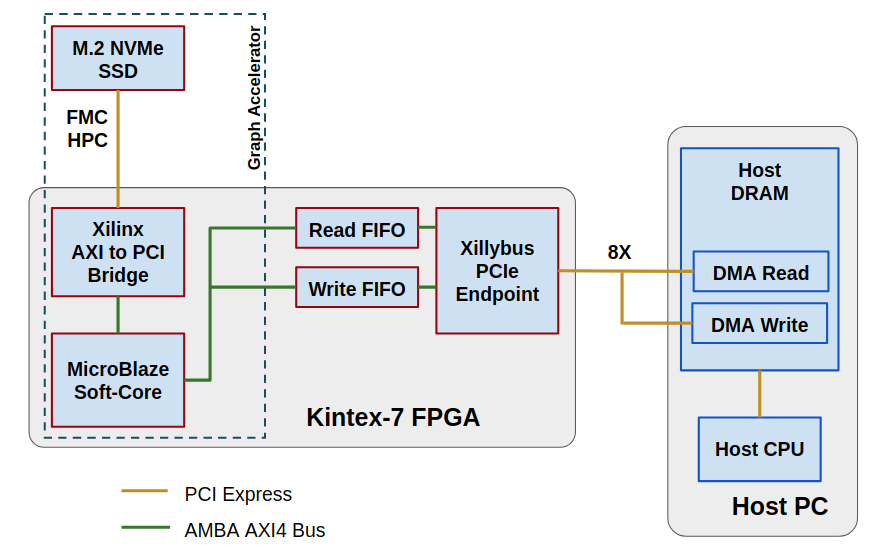
\includegraphics[scale = 0.4]{pic/HardwareConn.png}
  \caption{Hardware Connectivity Overview}
  \label{fig:hardware}
\end{figure}

% Figure
\begin{figure}[h]
  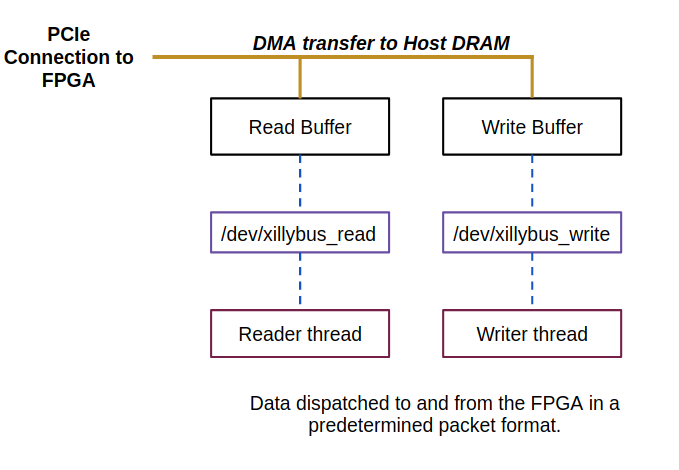
\includegraphics[scale = 0.4]{pic/HostCommunication.png}
  \caption{Host Communication Pipeline}
  \label{fig:host}
\end{figure}

\subsubsection{PetaLinux}
On the Kintex, the MicroBlaze soft-core processor runs Xilinx's PetaLinux distribution.  A Linux driver for the SSD interface IP core has been made available by Opsero.  The graph management routines access the graph data stored on SSD using typical Linux system calls.

\subsubsection{Linux Operating System}
Xillybus supports both Linux and Windows hosts.  Some Linux distributions (such as Ubuntu 14.04 and later) prepackage the driver.  Operation of the Kintex-7 as a PCIe endpoint has been verified on Ubuntu Linux 16.04.  The host can run any Linux distribution on which the Xillybus driver can be installed.

\subsection{Experimental Platform Overview}
The Kintex-7's PCI-Express edge connector is plugged into an available PCIe slot (with minimum 8x width) on the host PC's mainboard.  This connects the XillyBus IP as an Endpoint to the PCIe bus and allows communication with the driver on the host PC.  

In the Kintex's FPGA fabric, the Xillybus IP is connected via AXI4 Stream bus to FIFOs which in turn connect to a DMA core.  At the request of the Kintex's processing system (MicroBlaze), the DMA core can mark two areas of onboard DDR3 RAM to send and receive data to and from the host PC.  Because the MicroBlaze system is connected to the Xillybus IP only through memory, it is free to act as a PCI Root Complex of its own, connected to the SSD by a separate bus to serve its storage needs.

Figure \ref{fig:Vivado} is the final simplified block diagram of our design in Vivado.  The green components form the Xillybus connection to the host.  Its 32-bit input and output AXI Stream ports are connected via FIFOs to a DMA block which faces main memory.  The 8-bit stream ports are looped back for internal testing purposes.  The FIFOs also serve to isolate the Xillybus core, which by design exists in a different clock domain from the rest of the system.  The purple lines and components illustrate the MicroBlaze's connection to the SSD.  Finally, the bright blue lines indicate the MicroBlaze and the SSD controller's connection to main memory.

% Figure
\begin{figure}[h]
  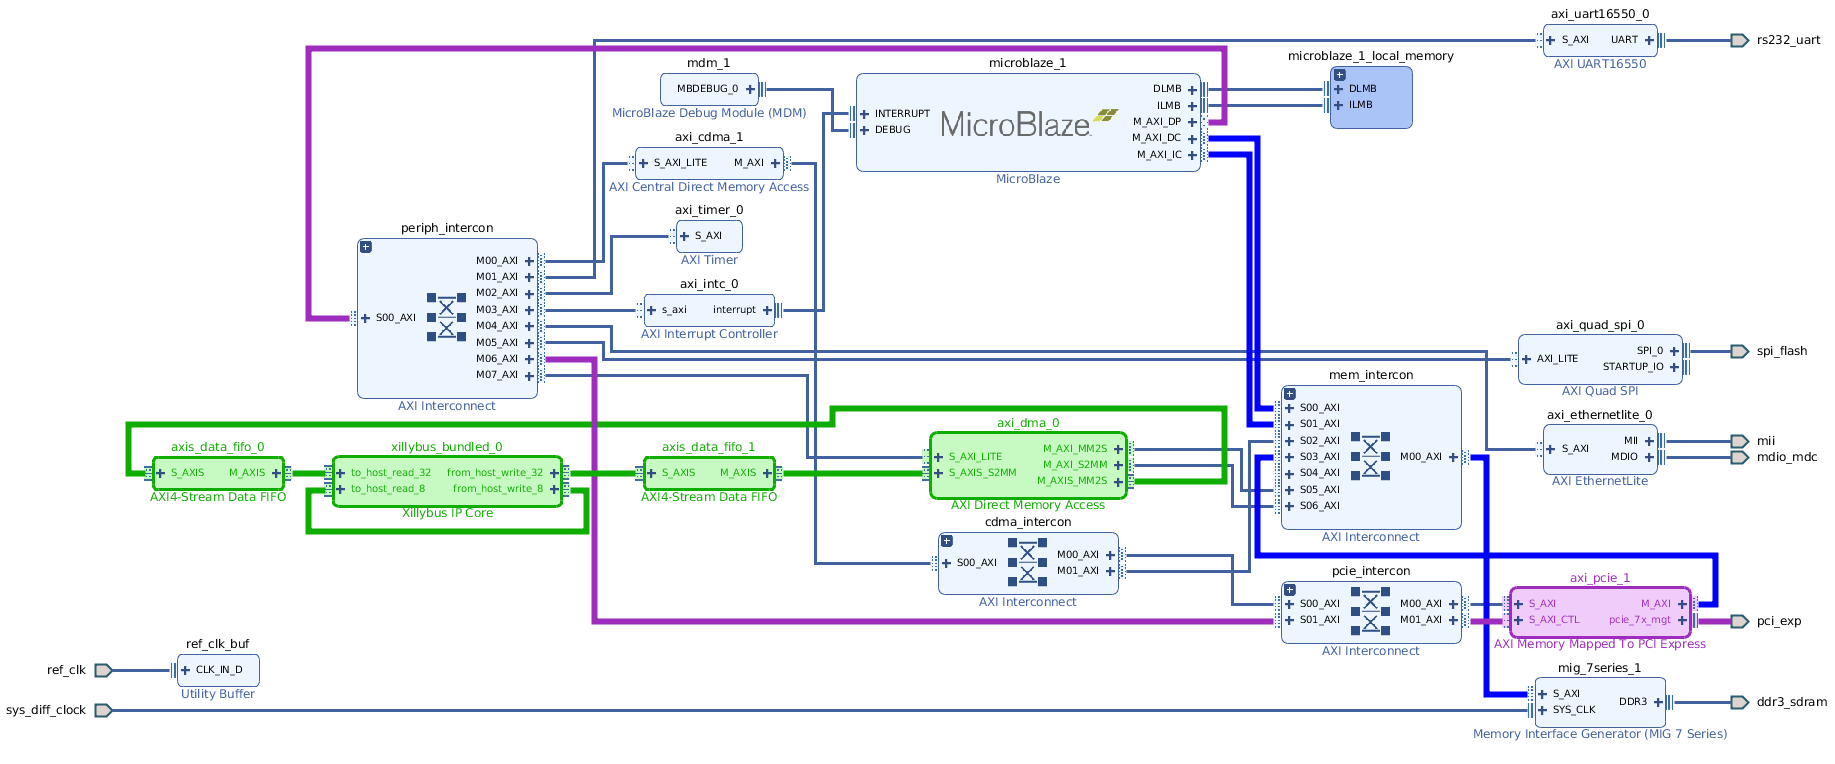
\includegraphics[width=\textwidth,keepaspectratio]{pic/block.png}
  \caption{Vivado Block Design}
  \label{fig:Vivado}
\end{figure}

\subsection{Implementation Results}

The connection between MicroBlaze and SSD was found to be significantly slower than expected.  Whereas this Samsung 950 Pro is advertised as achieving speeds of close to 1 Gbit/s writing and 2.5 Gbit/s reading, our tests writing and reading data from memory to SSD took minutes to complete where they should have taken seconds.  One major issue is the latency of a soft-core system running a full-featured operating system.  Another potential issue is the fact that the PCI bus and the CPU both share the same connection to memory, where the CPU's instructions are stored.  This bus sharing leads to a bottleneck that limits execution speed.  Ideally, this can be fixed by developing graph processing logic that interfaces directly in hardware with the SSD, and is a direction for future work.

The Xillybus PCIe connection was proven reliable and fast, achieving speeds of over 500 MB/s in our transfer speed tests.

The ability to interface the MicroBlaze with the Xillybus IP via the DMA/FIFO bridges was verified using user space memory mapping (i.e., \emph{mmap()} calls) to perform loopback communication on the 8-bit lines.

Although the 7-series FPGA are designed for high-speed PCIe communication with a host, we discovered a severe limitation.  There is only one physical PCIe device block available to the Kintex-7's FPGA fabric.  This means that, regrettably, it is impossible to integrate the system as designed.  There are a few options to move forward with this project.  

One method is to reconfigure the MicroBlaze as an Endpoint and use Bus Mastering for SSD communications.  However, this approach implies a significant performance hit as the ultimate purpose of this platform is to enable continuous streaming graph computation.  Another method is to use a different communication method with host other than PCIe, such as Ethernet or Serial communications.  This would also result in a high communication latency.

Another method still is to change to the Virtex-7 FPGA, which, depending on specific model, possess at least two PCIe device blocks, making multiple PCI buses possible.  The drawback to this approach is cost, but is perhaps the most robust solution for our purposes.


\section{Graph Per-processing}
Graph pre-processing, an integral part of nearly every graph traversal or transformation algorithm, has drawn renewed attention recently \cite{malicevic2017everything}. One form of pre-processing translates raw graph structured data (e.g., edge lists) to other formats, like adjacency lists.  There are two standard raw data layouts: vertex-centric and edge-centric.  The format of the data impacts the computational efficiency of graph traversal methods.  Most research works are based on already pre-processed data . The pre-processing time for graph computing often ignored when compare with the benefits of proposed algorithmic optimization with other method. Figure~\ref{fig:1} illustrates the significance of pre-processing time. For example, graph (c) in Figure~\ref{fig:1} shows the actual run-time of a sparse-matrix vector multiplication using adjacency lists is significantly slower than using a simple edge array when the time to generate the adjacency list is considered.



Some algorithms do not require pre-processing of data.  XStream \cite{roy2013x} is one them.  X-Stream is novel in that it employs an edge-centric approach in favor of a vertex-centric which dramatically reduces pre-processing requirements.   Also, it streams completely unordered edge lists rather than performing random access.  This leverages the fact that bandwidth for sequential access for all storage media is higher than that of random access.

GraphAcc can be used for graph per-processing. In this research challenge, we can have a Near Data computing based per-processing device tp help us save the computation time. 


This degree distribution is detrimental for graph computing because vertex degree is closely related to the amount of workload that is binding to this vertex. For instance, in BFS, iBFS, PageRank, SSSP, k-Core, WCC and SpMV, the amount of neighbors is exactly the number of workloads. Therefore, balancing workload across threads, machines or SSDs is crucial.

% Figure
\begin{figure}[h]
  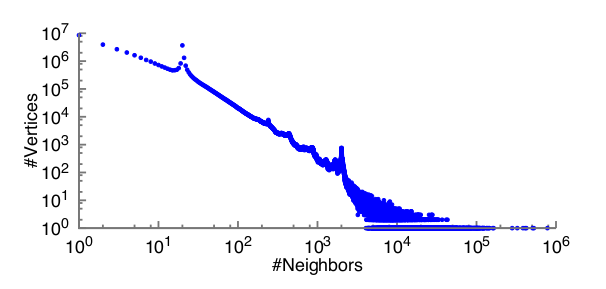
\includegraphics[scale = 0.3]{pic/powerdistribution.png}
  \caption{Degree distribution of Twitter Graph}
  \label{fig:power}
\end{figure}

One of the challenges for GraphAcc is to handel this highly skewed workload distribution.  

\section{File system} 
One trend in modern operating systems is to issue IOs in larger sizes, e.g., 4KB by default in some Linux distributions. While this approach is used to achieve high sequential bandwidth from underlying storage devices like hard drives. However, graph algorithms inherently issus small data requests. One can see that most (99\%) of IO requests are much smaller than 4KB. 
% Figure
\begin{figure}[h]
  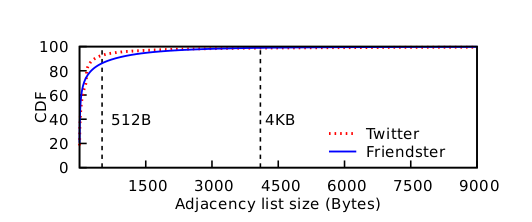
\includegraphics[scale = 0.3]{pic/DistribtionIO.png}
  \caption{Distribution of IO sizes}
  \label{fig:iodistribution}
\end{figure}
We choose to use a small IO size of 512 bytes as the basic block for graph data IOs. Fortunately, new SSDs are capable of delivering good IOPS for 512-byte read requests for both random and sequential IOs.

\section{Conclusion}
In this report, I have present several improvement for my research in the future. 

% Bibliography
\bibliographystyle{ACM-Reference-Format}
\bibliography{bibliography_ACA}




\end{document}
